\chapter{Theory of atomistic representations}
\label{sec:atomistic_representation}

This chapter covers the theory and the computation of symmetrized features on the atomic-scale.
%The methods presented have been historically developped incrementally improving fferent aspects in the computation of the 
%advantage of mathematical tricks to compute efficiently features, the connection between those has been much later.
%We take an approach similar to \cite{willatt2019atom} defining summarizing all approaches 
A similar approach as in Ref.~\cite{willatt2019atom} is taken into the theory of atomistic represantions utilizing concepts that exists in representation theory.
We therefore first introduce different functional forms $f:V\rightarrow\mathbb{R}$ representing the atomic structure $A$.
On these functional forms a set of functions $\{b_k:V\rightarrow\mathbb{R}\}_{k=1}^{M}$, the \emph{basis set}, is expanded
\begin{equation}
  \int_V\mathrm{d}\mathbf{q}\, f(\mathbf{q})b_k(\mathbf{q}) = c_k
\end{equation}
to obtain a set of \emph{expansion coefficients} $\{c_k\in\mathbb{R}\}_{k=1}^{M}$ that can be used to build a model mapping the coefficients to phyisical properties like energy and forces.
The choice of the functional form as well as the basis set is essential for an effective description, i.e. a description that captures information with the least amount of number coeffients. 
Prior knowledge about physical properties and distributions of atomic structures is used to bias the construction to more effective descriptions in the field.
A family of representations based on the higher orders of the \emph{atomic density} function is introduced and it is shown how invariances are embedded efficiently.
%\emph{atom-centered density correlation} (ACDC) function representing the atomic structure as correlation between local atomic densities is introduced and its connection to widely established descriptors is shown.
Furthermore, general characteristics of basis functions used in the field of atomic-scale modelling and how to efficiently embed invariances into these are presented.
\begin{figure}
    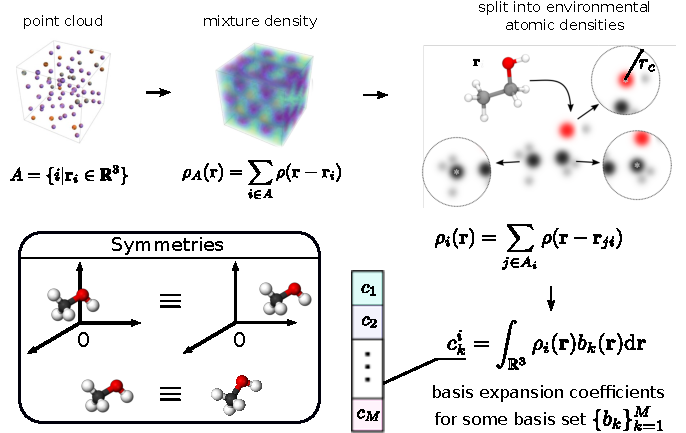
\includegraphics[width=\textwidth]{fig/atomistic_repr_schematic.pdf}
    \caption{A schematic showing the construction of features as input for a statistical inference model based on the atomic-centered density correlations function. The figure of the atoms in the box are retrieved from Ref.~\cite{noh2019inverse}. The figure of the atomic environments is retrieved from Ref.~\cite{willatt2019atom}. The methanol molecule is retrieved from Ref.~\cite{wiki:Alcohol_(chemistry)}.}
    \label{fig:acdc-scheme}
\end{figure}

%In the following methods of encoding the information present in the symmetrized many-body correlation function in Eq.~\ref{eq:invariant_many_body_correlation_function} into a vector representation are presented.

%By separating the atomic structure descriptor into descriptors for atomic environments different methods for constructing a structural descriptor out of atomic environment contributions have been proposed.

%% add maybe the fingerprint in zhu2016fingerprint based on local overlap matrix
\section{Atomic-centered density}
%Based on the successfully used assumption that the atomic nuclei can be
%treated classically, we can directly use the geometric information of the
%atomic nuclei.  and  used in Born-Oppenheimer and Car-Parinello molecular
%dynamics simulation Breaking down atomic structure wavefunction into atomic
%positions is rationalized by the Born-Oppenheimer approximation treating
%nuclear and electron wavefunction separately due to their large difference in
%mass.
%% TODO read the KS paper again, there should be a reasoning for the atomic structure potential to the energy
%Another assumption done in Born-Oppenheimer and Car-Parinello molecular
%dynamics is to treat the nucleus classical, thus the a full representation of
%the atomic structure by the positions of its nuclei and their chemical species
%exist.  Furthermore, in contrast to the previous approach, a continuous
%function exists mapping the positions of the atoms to a physical property of
%the atomic structure.
%%Furthermore, the nuclei and treating the nuclei classically, the atomic structure can be fully represented by the positions of its nuclei and their chemical species.
%%Furthermore, in this framework a continuous function exists mapping these information to a physical property.
%As a consequence efficient encapsulation of geometric information of atomic
%structures into a descriptor has dominated recent development of descriptors
%in the atomic scale\cite{willatt2019atom}.  TODO maybe Within the
%Car-Parinello framework
%To this end several methods have been proposed to incorporate into a descriptor transformations under which the target atomic properties are equivariant\cite{willatt2019atom}.
%%and for models\cite{schutt2018schnet} have been proposed.
%For scalar properties, these transformations are rotations and translations of
%the atomic structure, and permutations of the atom order.  From a statistical
%learning theory perspective the incorporation of invariances into the
%descriptor can be seen as a reduction of the hypothesis class in size
%% and in the model case as the introduction of prior knowledge into the model.
%~\cite{willatt2019atom}.
A majority of developed atomistic descriptors can be seen as different approaches in describing the same function representing the atomic structure in different ways, the atomic density\cite{willatt2019atom} 
\begin{equation}
  \label{eq:basis_expansion}
  \rho(\mathbf{r}) = \sum_{i\in A} \rho(\mathbf{r}-\mathbf{r}_i),\quad \rho:\mathbb{R}^3\rightarrow\mathbb{R}
\end{equation}
where $\mathbf{r}_i\in\mathbb{R}^3$ is the position of the $i$th atom in the atomic structure $A$ and $\rho$ is an arbitrary function decaying from its origin. 
Commonly, the Gaussian $g$ or Dirac $\delta$ function are used for the density
$\rho$\cite{musil2021physics}.
A widely adapted approach to impose translational invariance, i.e. independence of the center of the structure, is to describe the atomic structure as a sum of local atomic environments
\begin{equation}
  \sum_{i\in A} \rho_i(\mathbf{r}) = \sum_{i\in A}\sum_{j\in A_i} \rho(\mathbf{r}-\mathbf{r}_{ji}),
\end{equation}
where $A_i$ is the set of all atoms that are in the \emph{environment} of atom
$i$, in most applications defined as the set of atoms within a certain distance, the
\emph{cutoff}. Further, $\mathbf{r}_{ji}$ is the direction vector $\mathbf{r}_j-\mathbf{r}_i$. 
We call $\rho_i$ \emph{neighbor density}.
This approach aligns with the partition of the target property $y$ into atomic contributions
\begin{equation}
  \label{eq:structural_separation}
  \sum_{i\in A} y_i = y.
\end{equation}
This decomposition into local properties is motivated by the heuristical observation that atomic properties decay with their distance to the center, coined \emph{nearsightedness}\cite{prodan2005nearsightedness}.
%The exact meaning of this atomic contributions is still a reasearch question.
\section{Hierarchy of symmetrized representations}
%tensorial properties
%Learning tensorial properties requires change under rotation\cite{chemrev}.
%Cartesian tensors can be transformed to this basis using a set of rules\cite{cartesiantransformationTODO}
%Such equivariant behavior under rotation can be embedded by splitting the density function over the corresponding SO(3) subgroup.
%It is required to increase the higher-body orders and predicting tensorial properties to separate the density function into its irreducible spherical tensors 
%\begin{equation}
%\label{eq:integration_over_subgroup}
%%\ket{A^{(n)}}_{\hat{R}\hat{t}} = \int \mathrm{d}\hat{R}\,\int \mathrm{d}\hat{t}\, \bigotimes_{m=1}^n\hat{R}\hat{t}\ket{\mathcal{A}}
%  \ket{\mathcal{X}^{(\nu)}}_{\hat{R},h} = \int_{SO(3)} \hspace{-1em}\mathrm{d}\hat{R}\, \underbrace{\hat{R}\ket{\mathcal{X}}_h\otimes \cdots \otimes \hat{R}\ket{\mathcal{X}}_h}_{\nu-\text{times}}, %TODO change equation
%\end{equation}
As a large family of physical quantities are invariant under rotations of the atomic structure, it is needed to account for rotational invariance in the process of relating atomic structure to such quantities.
Rotational invariance can be embedded into the functional form by integrating over the rotation group $SO(3)$
\begin{equation}
\label{eq:integration_over_subgroup}
  f^1(\mathbf{r}) = \int_{SO(3)}\mathrm{d}\hat{R}\, \rho_i(\hat{R}\mathbf{r})
\end{equation}
and can be further extended to higher orders of the density
\begin{equation}
\label{eq:integration_over_subgroup_higher_order}
  f^\nu(\mathbf{r},\ldots, \mathbf{r}_\nu) = \int_{SO(3)}\mathrm{d}\hat{R}\, \rho_i(\hat{R}\mathbf{r}_1)\rho_i(\hat{R}\mathbf{r}_2)\ldots\rho_i(\hat{R}\mathbf{r}_\nu)
\end{equation}
named \emph{atom-centered density correlation} function\cite{nigam2022unified}.
While in principle this integral can be numerically evaluated, such an integration is not suitable to efficiently evaluate the expansion coefficients.
Hence, it is essential to chose suitable candidates for the density $\rho$ and the basis set $\{b_k\}_{k=1}^M$ that yield an analytical solution for the integral.
Note that post-symmetrization methods have recently been developed that also allow an efficient evaluation of the integral by averaging over all possible reference frames within a order $\nu$ tuple\cite{pozdnyakov2023smooth}, these are however not in the scope of the thesis.

\subsection{Ordered basis set}
%It has been shown that most representations can be derived naturally from atomic density by constructing higher-order correlations and imposing rotational invariance\cite{willatt2019atom}.
%Rotational invariance is obtained by taking the Haar integral of the function over the $SO(3)$ group, i.e. integrating over all 3D rotations.
An explicit solution of the integral over $SO(3)$ can be expressed for the Dirac $\delta$ densities.
Here we present solutions for order 1 and 2 that should make the idea clear
\begin{subequations}
\label{eq:dirac_delta_haar_integral}
\begin{align}
    \label{eq:dirac_delta_haar_integral_2body}
    \int_{SO(3)} \mathrm{d}\hat{R}\, \delta(\hat{R}\mathbf{r}-\mathbf{r}_{ji}) &\propto_r \delta(r-r_{ji}), \\% = f^1(r)\\
    %\langle r| \mathcal{X}_i\rangle_{\hat{R},g\rightarrow\delta} &\propto \sum_{j\in\mathcal{X}_i}\delta(r-r_{ij}), \\
    \label{eq:dirac_delta_haar_integral_3body}
    %\langle rr'\theta | \mathcal{X}^{(2)}_i\rangle_{\hat{R},g\rightarrow\delta} &\propto \sum_{j,k\in\mathcal{X}_i} \delta(r-r_{ij})\delta(r-r_{ik})\delta(\theta-\theta_{ijk}),
    \int_{SO(3)} \mathrm{d}\hat{R}\, \delta(\hat{R}\mathbf{r}-\mathbf{r}_{ji}) \delta(\hat{R}\mathbf{r}^\prime-\mathbf{r}_{ki}) &\propto_r \delta(r-r_{ji})\delta(r^\prime-r_{ki})\delta(\theta-\theta_{jki}). %= f^2(r, r, \theta)
\end{align}
\end{subequations}
We use $\propto_r$ to ommit radial terms $r$ that appear due to the integration in $3$-dimensional space and are not essential as typically a radial scaling term is added to the functional form to control the general scaling.
The correlation function of order 2 naturally results in a description of distance to atom $i$ and the order 3 function in the two distances and an angle wrt. atom $i$.
Here we use $\propto_r$ to ignore any radial factors that appear.
One approach to obtain a numerical description from this function is based on the concatenation of discrete information of the nonzero values in Eqs.~\ref{eq:dirac_delta_haar_integral} to an ordered $n$-tensor e.g. pairwise distances\cite{rupp2012fast, montavon2012learning, montavon2013machine, sadeghi2013metrics}, 3-body angles, 4-body torsions\cite{huang2016communication}.
%%\begin{equation}
%%[f(\ket{\mathcal{A}\otimes\mathcal{A}\rangle},\ket{\mathcal{A}\otimes\mathcal{A}\rangle})]_{ij}
%%% can generalized to environments
%%\end{equation}
%%\begin{equation}
%%    C_{ij} = \langle r_i r_j|\mathcal{X}^{(n)}\rangle
%%    \langle r_1\ldots r_{n^2}|\mathcal{X}^{(n)}\rangle
%%\end{equation}
To achieve permutational invariance the sorted eigenvalues\cite{rupp2012fast, sadeghi2013metrics, zhu2016fingerprint} or sorted tensor entries\cite{hansen2015machine, barker2016localized, huang2016communication} have been used.
For the pairwise distances it has been shown that both approaches for permutational invariance suffer from degeneracies, mapping different atomic structure to the same descriptor\cite{moussa2012comment}.
A solution to avoid these degeneracies has been to sum over random permutations of the matrix\cite{montavon2012learning, montavon2013machine, sadeghi2013metrics}.
While this approach works for small molecules, it does not scale well with the number of atoms.
A still computational very costly but feasible solution is to find a canonical permutation for all environments in the data set by constructing a transitive closure of all bi-partite permutations\cite{chmiela2018towards}. The bi-partite permutations are determined by solving the matching problem between the principal eigenvectors of two matrices with the Hungarian algorithm\cite{kuhn1955hungarian}, the transitive closure is constructed with a minimum spanning tree.
Although it has been shown that for regression tasks other descriptors lead to more accurate results\cite{de2016comparing, bartok2017machine, jager2018machine}, still comparable results have been reached with a local atomic environment version of the sorted pairwise distances matrix\cite{barker2016localized} and a sorted 4-body torsion tensor\cite{huang2016communication}.

\subsection{Fixed basis set}
%%\[\langle\mathbf{r}\mathbf{r'}|{\mathcal{A}\otimes\mathcal{A}}\rangle = \sum_i g(\mathbf{r}-\mathbf{r}_{ij})\]
%The use of projections of the symmetrized many-body correlation function has been one of the early ways to construct a descriptor.
As the concatenation of the coefficient results in noncontinuous descriptions, a problem that arises from keeping varying the basis set for each sample, a natural solution is to expand on the function with a fixed basis set that is used for all environments\cite{behler2011atom,bartok2013representing,drautz2019atomic}.
By expanding with a basis function for different orders one obtains coefficients of the form
\begin{subequations}
\label{eq:dirac_delta_expansion_coeffs}
\begin{align}
    \label{eq:dirac_delta_expansion_coeffs_2body}
    b_k(r_{ji}) &\propto_r\int_{\mathbb{R}^3}\mathrm{d}\mathbf{r}\, b_k(r)\delta(r-r_{ji})\\
    \label{eq:dirac_delta_expansion_coeffs_3body}
    b_k(r,r\prime,\theta_{jki})&\propto_r\int_{\mathbb{R}^3\times\mathbb{R}^3}\mathrm{d}\mathbf{r}\mathrm{d}\mathbf{r}^\prime\, b_k(r,r\prime,\theta_{ijk})\delta(r^\prime-r_{ji})\delta(r-r_{ki})
    \delta(\theta(\mathbf{r}\mathbf{r}^\prime) - \theta_{jki}) 
    %\delta(\hat{\mathbf{r}}\cdot\hat{\mathbf{r}}^\prime - \hat{\mathbf{r}}_{ji}\cdot\hat{\mathbf{r}}_{ki})
\end{align}
\end{subequations}
%to obtain a continuous description\cite{behlerparinello}.
%As example two types of basis functions the atom-centered symmetry functions (ACSFs)\cite{behler2011atom}
%The main characteristics of the these functions can be seen in the following examples
%
%\begin{subequations}
%\begin{align}
%G_2(r) &=  \exp(\eta(r-r_s)^2), \\
%%original form
%%G_4(\theta, \mathbf{r}) &= 2^{1-\eta} (1+\lambda \cos(\theta))^{\zeta} \exp(-\eta\|\mathbf{r}\|^2),
%G_4(r, r',\theta) &= 2^{1-\zeta} (1+\lambda \cos(\theta))^{\zeta} \exp(-2\eta(r^2+r'^2 -rr'\cos(\theta))),
%\end{align}
%\end{subequations}
%where $r_s$, $\lambda,\zeta$ and $\eta$ are parameters which are chosen \textit{a priori} computation.
%The expansion coefficients are computed by expanding on the Diral $\delta$ density
%\begin{subequations}
%  \label{eq:symmetry_function_as_projection}
%  \begin{align}
%    %\langle G_2|\mathcal{X}_i\rangle_{\hat{R},g\rightarrow\delta} &= \sum_{j\in\mathcal{X}_i} G_2(r_{ij})\\
%    \int G_2(r)\delta(r-r_{ij}) \,\mathrm{d}\mathbf{r} &\propto G_2(r_{ij})\\
%    %\langle G_4|\mathcal{X}_i^{(2)}\rangle_{\hat{R},g\rightarrow\delta} &= \sum_{j,k\in\mathcal{X}_i} G_4(r_{ij},r_{ik}, \theta_{ijk}),
%    \int G_4(r,r\prime,\theta_{ijk})\delta(r-r_{ij})\delta(r-r_{ik})\delta(\theta-\theta_{ijk}) \,\mathrm{d}\mathbf{r}\mathrm{d}\mathbf{r}^\prime &\propto G_4(r_{ij},r_{ik}, \theta_{ijk})
%  \end{align}
%\end{subequations}
For order 1 an analytical solution of the integral in Eq.~\ref{eq:integration_over_subgroup} can be solved exploiting properties of the Gaussian function\cite{musil2019machine}
\begin{equation}
  \label{eq:order1_analytical_solution}
  \int_{SO(3)} \mathrm{d}\hat{R}\, g(\hat{R}\mathbf{r}-\mathbf{r}_{ji}) 
  %\propto_r \sinh(\frac{rr_{ji}^2}{2\sigma^2})\exp(-\frac{r^2+r_{ji}^2}{4\sigma^2}) \approx \exp(-\frac{r^2+r_{ji}^2}{4\sigma^2})
  %= 8\pi^2 \sinh(rr_{ji}^2/2\sigma^2)(rr_{ji}/2\sigma^2)\exp(-(r^2+r_{ji}^2)/4\sigma^2)
\end{equation}
%An expansion for er density functions requires results from angular momentum theory to solve the integral.
Solving the integral for higher orders or other densities requires more complex mathematical results.% from angular momentum theory\cite{yutsis1965theory}.
%egral s usually solved by expressing the density as a product of a radial and angular function
%\begin{equation}
%  \label{eq:radial_angular_density}
%  \rho(\mathbf{r}) = \rho_r(r)\rho_{\hat{\mathbf{r}}}(\hat{\mathbf{r}})
%\end{equation}
%which requires rotational symmetry of the density $\rho(\hat{R}\mathbf{r}) = \rho(\mathbf{r})$ as it is for the Gaussian function. % or Coulomb potential. %Student's t-distribution.
%Since asymetric densities typically are integration, it is not a restrictive constraint.
As spherical harmonics $Y_\mu^\lambda(\hat{\mathbf{r}})$ have been studied extensively in invariant theory\cite{dowker2008spherical} it is a suitable candidate to solve the integral in Eq.~\ref{eq:integration_over_subgroup_higher_order}.
To take advantage of the results in angular momentum theory\cite{yutsis1965theory}, the density needs to be reexpressed as a combination spherical harmonics.
Consequently, for a complete basis of the density a radial basis is needed $\{R_n(r) :\mathbb{R}\rightarrow\mathbb{R}\}$ to cover the radial part of the density.
%For simplicity in the derivation we impose orthogonality on $R_n(r)$,
Then density can thus be reformulated as
\begin{equation}
  \label{eq:radial_angular_density}
  \rho_i(\mathbf{r}) = \sum_{n\lambda\mu} c_{n\lambda\mu}R_n(r)Y^\lambda_\mu(\hat{\mathbf{r}}).
\end{equation}
%\begin{equation}
%  \rho(\mathbf{r}) = \sum_{n\lambda\mu}R_n(r)Y^\lambda_\mu(\hat{\mathbf{r}})
%\end{equation}
We will solve Eq.~\ref{eq:integration_over_subgroup_higher_order} for order 2 omitting the radial part for simplicity
%\begin{subequations}
%  \rho(\mathbf{r}) = \sum_{\lambda\mu} \rho_{\lambda\mu}(\mathbf{r}).\\
%  \rho_{\lambda\mu}(\mathbf{r}) = \int\mathrm{d}\mathbf{r}\, \rho(\mathbf{r})Y^\lambda_\mu(\hat{\mathbf{r}})
%\end{subequation}
\begin{subequations}
  \label{eq:solving_haar_integral}
\begin{align}
  &\sum_{\lambda\lambda^\prime\mu\mu^\prime}\int \mathrm{d}\hat{R}\, Y^{\lambda}_\mu(\hat{R}\hat{\mathbf{r}})Y^{\lambda^\prime}_{\mu^\prime}(\hat{R}\hat{\mathbf{r}}^\prime)\\
  & = \sum_{\lambda\mu} \int \mathrm{d}\hat{R}\, Y^\lambda_\mu(\hat{R}\hat{\mathbf{r}})Y^\lambda_{\mu}(\hat{R}\hat{\mathbf{r}}^\prime) \quad \textrm{(orthogonality spherical harmonics)}\\
  & = \sum_{\lambda\mu} \int \mathrm{d}\hat{R}\, \sum_{k}D_{\mu k}^\lambda(\hat{R})Y^\lambda_k(\hat{\mathbf{r}})\sum_{k^\prime}D_{\mu k^\prime}^\lambda(\hat{R})Y^\lambda_{k^\prime}(\hat{\mathbf{r}}^\prime) \quad \textrm{($\mathbf{D}(\hat{R})$ is the Wigner D-matrix)}\\
  & = \sum_{\lambda} Y^\lambda_k(\hat{\mathbf{r}})Y^\lambda_{k^\prime}(\hat{\mathbf{r}}^\prime)\int \mathrm{d}\hat{R}\, \sum_{\mu kk^\prime}D_{\mu k}^\lambda(\hat{R})D_{\mu k^\prime}^\lambda(\hat{R})\\
  %& = \sum_{\lambda} \int \mathrm{d}\hat{R}\, \sum_{kk^\prime}\delta_{kk^\prime} Y^\lambda_k(\hat{\mathbf{r}})Y^\lambda_{k^\prime}(\hat{\mathbf{r}}^\prime) \quad \textrm{(orthogonality Wigner D-matrix)}\\
  % https://en.wikipedia.org/wiki/Wigner_D-matrix#Orthogonality_relations
  & = \sum_{\lambda} \sum_{kk^\prime}\delta_{kk^\prime} Y^\lambda_k(\hat{\mathbf{r}})Y^\lambda_{k^\prime}(\hat{\mathbf{r}}^\prime) \quad \textrm{(orthogonality Wigner D-matrix)}\\
  & = \sum_{\lambda k} Y^\lambda_k(\hat{\mathbf{r}})Y^\lambda_{k}(\hat{\mathbf{r}}^\prime)
\end{align}
\end{subequations}
Incorperating the radial part into the above derivation we obtain
\begin{equation}
  %\sum_{nn^\prime\lambda}\int \mathrm{d}\hat{R}\, R_n(r)Y^\lambda_\mu(\hat{R}\hat{\mathbf{r}})R_{n^\prime}(r^\prime)Y^\lambda_\mu(\hat{R}\hat{\mathbf{r}}^\prime) \propto 
  \sum_{nn^\prime} R_n(r)R_{n^\prime}(r^\prime) \sum_{\lambda\mu} Y^\lambda_\mu(\hat{\mathbf{r}})Y^\lambda_{\mu}(\hat{\mathbf{r}}^\prime)
\end{equation}
This retrieves the well known representation named \emph{smooth overlap of atomic positions}\cite{bartok2013representing}.
%What has been used is that rotations applied on spherical harmonics results in a linear combination which coefficients are represented by the Wigner D-matrix $D_{mm^\prime}^l$ as well as the orthogonality of Wigner D-matrices.
A solution for the order 3 can be further retrieved using the fact that the product of Wigner D-matrices can be decomposed into a linear combination of Wigner D-matrices
\begin{equation}
  D^{l_1}_{m_1m_1^\prime}(\hat{R})D^{l_2}_{m_2m_2^\prime}(\hat{R}) = \sum_{\lambda m m^\prime} D^{\lambda}_{\mu m^\prime}(\hat{R}) (C^{\lambda l_1l_2}_{\mu m_1m_2})C^{\lambda l_1l_2}_{mm_1^\prime m_2^\prime}
  %TODO I need to write somewhere that real spherical harmonics are considered here
\end{equation}
where $C^{\lambda l_1l_2}_{\mu m_1m_2}$ are the Clebsch-Gordan coefficients\cite{yutsis1965theory}.
This relationship was first used in Ref.~\cite{bartok2013representing} to produce order 3 functions, often referred to as \emph{bispectrum} and has later been put into a recursive formula to create expressions for higher-order functions with different approaches for the compression of the basis set in the high-dimensional space\cite{kondor2018clebsch,yan2019fourier,nigam2020recursive}
\begin{equation}
  \label{eq:recursive_higherorder}
  f^{\nu+1}(\mathbf{r}^{\nu+1}) = \sum_{k} c_k f_k^\nu(\mathbf{r}^{\nu})f_k^1(\mathbf{r})%\sum_{\mu m}C^{\lambda l_1l_2}_{\mu m_1m_2} f_\nu(r^{\nu})f(\mathbf{r})
\end{equation}
%A key problem in propagation to higher orders is to find a suitable basis set that represents higher order space effectively has been solved in several ways\cite{kondor2018clebsch,yan2019fourier,nigam2020recursive}.
Another reason for the choice of spherical harmonics as bases is the fact that they form an irreducible representation of $SO(3)$, thus they cannot further compressed without some information loss when expanded on a general function on a surface of a sphere. %TODO into what
While a reducible basis as \emph{moment tensor potential}\cite{shapeev2016moment} results in lower accuracies, it also leads to a faster evaluation time\cite{zuo2020performance,xie2023ultra}. %TODO reformulate this
% such that they reach accuraciesthat are sufficient for applications while operating on a much faster level\cite{zuo2020performance,xie2023ultra}.
%Further results from Ref.~\cite{yutsis1965theory} results us to u%TODO is this true 

%\subsubsection{Angular basis}
%Spherical harmonics $Y_l^m$ form an irreducible representation of $SO(3)$, i.e. cannot be decomposed into smaller more compact representation.
%They are therefore an obvious candidate to model equivariances with a wide adoption in the field\cite{bartok,TODO}.
%%While there are other candidates exists, it is TODO check out MTP how they build ivariant representation
%
%Bases beneficial wrt. an efficient solution to the Haar integration separate the ACDC into a radial and an angular contribution represented by spherical harmonics.
%The integral over the rotation group for 3-body interaction can then be resolved into linear combinations of correlations of spherical harmonics\cite{bartok2013representing}
%\begin{equation}
%    \langle l| \mathcal{X}^{(2)}\rangle_{\hat{R}} \propto \frac1{\sqrt{2l+1}} \sum_{m=-l}^l (-1)^m \langle lm|\mathcal{X}\rangle  \langle l-\hspace{-0.2em}m|\mathcal{X}\rangle.
%\end{equation}
%
%Due to the $Y_l^m$ being irreducible representation of SO(3), they are enforced for
%modeling equivariances and cannot be decomposed into smaller more compact description
%to model space. There is still a
%degree of freedom by chosing the $l$ channels and their size per $n$ channel,
%but a compression between $l$ channels makes preservance of equivarance in the
%best case complicated and in the worst unrecoverable.

%For the radial contribution commonly a radial basis functions $R_n$ is used separating the radial part from the spherical harmonics $Y^l_m$\cite{bartok2013representing},
\subsubsection{Basis expansion}
As the derivation in Eq.~\ref{eq:solving_haar_integral} shows that the evaluation of the integral results in a product sum of radial and angular components.
A natural choice for a basis function is choosing $B_{nn^\prime\lambda}(\mathbf{r},\mathbf{r}^\prime) = R_n(r)R_{n^\prime}(r^\prime)\sum_\mu Y_\mu^\lambda(\hat{\mathbf{r}})Y_\mu^\lambda(\hat{\mathbf{r}}^\prime)$.
The order 2 expansion coefficients then decomposes into the spherical expansion coefficients
\begin{subequations}
\begin{align}
    \label{eq:gaussian_expansion}
    c_{n\lambda\mu} &= \int\mathrm{d}\mathbf{r} R_n(r)Y_\mu^\lambda(\hat{\mathbf{r}})\rho(\mathbf{r}),\quad\textrm{spherical expansion coefficients}\\
    \label{eq:soap_expansion}
    \sum_\mu c_{n\lambda\mu}c_{n^\prime \lambda\mu} &= \int\mathrm{d}\mathbf{r}\mathrm{d}\mathbf{r}^\prime\, B_{nn\prime\lambda}(\mathbf{r}, \mathbf{r}^\prime) R_n(r)R_{n^\prime}(r^\prime)\sum_{\lambda k} Y^\lambda_k(\hat{\mathbf{r}})Y^\lambda_{k}(\hat{\mathbf{r}}^\prime)
\end{align}
\end{subequations}
From the choice of the basis set for the neighbor density in Eq.~\ref{eq:radial_angular_density} a candidate for order 2 naturally derives that can be constructed from the initial spherical expansion coefficients.
Including the recursion in Eq.~\ref{eq:recursive_higherorder} into the consideration it becomes apparent that all higher order correlations can be constructed from one expansion.
This fact %that the propagation to higher-body orders does only require an expansion of the order 1 terms 
has been coined \emph{density trick}.
It moves the computation from evaluating the basis expansions for $(\nu+1)$-tuples as it shown in Eqs.~\ref{eq:dirac_delta_expansion_coeffs_3body} for oder 2 to computing the tensor products between the expansion coefficients of order $\nu$ as indicated the derivation in Eq.~\ref{eq:soap_expansion}.
Increasing the body-order from the expansion coefficients of order $\nu$ to $\nu+1$ scales as $O(NM+M^{\nu})$ while a direct expansion of the higher-order function scales as $O(M^{\nu+1}N^{\nu+1})$\cite{goscinski2021role}.
As example the costs for order 2 features in Eq.~\ref{eq:soap_expansion} without using the density trick the computation of the features for one atomic environem requires the expansion of $O({N\choose 3}) = O(N^3)$ triplets for each of the $M$ basis functions resulting in a total time complexity of $O(M^2N^3)$.
With the density trick one has to compute the expansion coefficients for the density $O(MN)$ to then to increase the order by a contracted tensor product scaling with $O(M^2)$ resulting a total time complexity of $O(MN+M^2)$.
%One has to be aware that this comparison considers the scaling behavior of two different factors the number of neighbors $N$ and the number of basis functions $M$.
Even though the scaling favors the use of the density trick, when embedding splines into the computation of the features, the slower iteration over all $(\nu+1)$-body parts can be balanced out by omitting the computational cost of tensor product and the model as shown in Ref~.\cite{xie2023ultra}.
This point will be discussed in more detail in Chapter~\cite{sec:splining}.
\subsubsection{Radial basis set}
\label{sec:radial_basis_set}
The radial basis function is a one dimensional function on a compatact domain $R_n:[0, r_c]\rightarrow\mathbb{R}$ determined by the cutoff $r_c$ forming one hyperparameter.
In the literature several radial basis functions have been proposed as shifted-Gaussians\cite{bartok2013representing}, Chebyshev polynomials\cite{shapeev2016moment,drautz2019atomic} or Gaussian type orbitals\cite{musil2021efficient} that all share certain characteristics to shown having positive effects on learning performance. 
One of these characteristics is the decay of the density with respect to the radial distance 
%incorperated in the functional form by multiplying smooth cutoff function $s(r):\mathbb{R}\rightarrow\mathbb{R}$ as well as in the form of the basis function.
together with an increase in the spread of the density as it deemphasizes the importance of information far from the center motivated by the beforementioned principle of nearsightedness\cite{prodan2005nearsightedness}.
%with increased distance which is often incorperated by adding a radial dependency on the smearing $\sigma$i.
To decrease the redundancy of the basis, one imposes orthogonality of the basis
As the dot product is a natural choice for a similarity measure between basis functions it can be seen that orthogonality is a desired property reducing the redundancy between the basis functions
\begin{equation}
  \int\mathrm{d}\mathbf{r}b_k(\mathbf{r})b_{k^\prime}(\mathbf{r}) = 0,\textrm{ if orthogonal}.
\end{equation}
If the basis choice does not provide orthogonality by definition, it is often achieved after the computation of the basis expansion coefficients using Löwden orthogonalization\cite{PIELA2014e99}.
Another common decision is that the basis functions are spread to uniformly cover the interval $[0, r_c]$ as first unbiased guess on representing the radial space\cite{schutt2018schnet,dusson2022atomic}.
This can be proceeded by a subsequent optimization step of the basis exactly for the radial distribution of the dataset.
%The notion of completeness convering the whole function space
%covering the compact space which is often done by centering each basis on an equispaced grid in the interaval $[0, r_c]$.
%A detailed discussion on completeness can be found in Ref.~\ref{chemrevTODO}.
%\papercomment{
%Introduce here DVR, GTO, Bartok
%}
\subsubsection{Radial expansion}
An important result of the expansion in Eq.~\ref{eq:gaussian_expansion} is that it is decomposed into radial and angular expansion term
\begin{equation}
  \label{eq:radial_expansion}
  c_{n\lambda\mu} R_n(r)Y^\lambda_\mu(\hat{r}) = \underbrace{c_{n\lambda}R^{lambda}_n(r)}_{\textrm{radial expansion}} c_{\lambda\mu}\tilde{Y}^\lambda_\mu(\hat{r}).\\
\end{equation}
The radial basis function couples with the angular basis function which makes an analytic expression nontrivial.
One approach to avoid the cost of an numerical integration is to approximate the neighbor density as a decoupled radial and angular contribution\cite{caro2019optimizing} 
\begin{equation}
  \rho_i(\mathbf{r}) \approx \rho_i,r(r)\rho_{i,\perp r}(\hat{\mathbf{r}})
\end{equation}
%The decoupled Gaussian function used in the initial suggestion $g(r)=$.
Another approach is to chose a radial basis that allows an analytical expression as Gaussian type orbitals\cite{musil2021efficient}.
The analytical expression is nowadays further replaced by a spline of for each of the radial expansion coefficents $c_{n\lambda}$ allowing an evaluation at constant time.
Since the splining the radial expansion coefficients has been shown to be cost-efficient\cite{musil2021efficient}, costly optimizations of the radial expansion coefficients have entered the design space\cite{goscinski2021optimal,bigi2022smooth,lopanitsyna2023modeling}.
These points are discussed in more detail in Chapter~\ref{sec:splining} about splining.

%only possible for certain radial basis as Gaussian type orbitals\cite{musil2021efficient}.

%Since the angular basis has its natural choice in the spherical harmonics, most optimization methods consider the radial expansion
%An approach that improves the effiency of the evaluation of this integration.
%\papercomment{Here I can put Caro's approach of decoupled atomic density. I can write later because the evaluation of the radial basis becomes so cheap by splining, we can get more accurate representation without additional cost in the prediction phase.}\\
%\papercomment{here I could talk about MTP but not so relevant}


%%Other examples are which fall in this category are invariant polynomials OPTTODO guilio paper
%
%Another approach takes projections on distances and (dihedral) angles together with a kernel density estimation to smoothen the projections\cite{huo2017unified, faber2018alchemical}.
%As example, the many-body tensor representation (MBTR), defined as a real grid basis expansion of the following functions\cite{huo2017unified}
%\begin{subequations}
%\label{eq:mbtr}
%\begin{gather}
%g_2(r) = \sum_{j\in\mathcal{X}_i} g(r-r_{ij}),\quad
%g_3(\theta) = \sum_{j,k\in\mathcal{X}_i} g(\theta-\theta_{ijk}),\\
%g_4(\varphi) = \sum_{j,k,l\in\mathcal{X}_i} g(\varphi-\varphi_{ijkl}).
%\end{gather}
%\end{subequations}
%It can be also seen as projections of 
%%the symmetrized many-body order correlations of the atomic environment 
%$\ket{\mathcal{X}_i^{(\nu)}}_{\hat{R},\delta}$ by smoothen the Dirac $\delta$ functions in Eq.~\ref{eq:dirac_delta_haar_integral} to Gaussian functions $g$ after the Haar integral has been applied.
%This smoothen operation will be notated with $\delta\rightarrow g$ allowing to express the functions in Eq.~\ref{eq:mbtr} as
%\begin{subequations}
%\begin{gather}
%g_{2}(r) = \langle r | \mathcal{X}_i\rangle_{\delta\rightarrow g,\hat{R},h\rightarrow\delta}, \quad
%g_3(\theta) = \langle \theta |\mathcal{X}_i^{(2)}\rangle_{\delta\rightarrow g,\hat{R},h\rightarrow\delta},\\
%g_4(\varphi) = \langle \varphi |\mathcal{X}_i^{(3)}\rangle_{\delta\rightarrow g,\hat{R},h\rightarrow\delta}.
%\end{gather}
%\end{subequations}
%Unlike the ACSF the projections are orthogonal to each other, therefore forming a complete basis set for marginals of the symmetrized many-body order correlation function.
%However, due to the limitation to marginals these kind of descriptors are still undercomplete with respect to the whole function.
%
%A comparison made between ACSF and MBTR to predict the adsorption energy of hydrogen on the surfaces of \textrm{MoS2} and \textrm{Au} based nanoclusters shows that the two representation present similar regression results\cite{jager2018machine}.

%While its success has been shown with neural networks, there are no results supporting the application of these descriptors with kernel models.

%- hyperspherical harmonics expansion
%- radial basis function + spherical harmonics 
%- Tensor Moment
%More descriptive representations can be motivated by the observation that the aforementioned descriptors can be expressed as projections of the symmetrized many-body correlation function in Eq.~\ref{eq:invariant_many_body_correlation_function}.
%as expressed in Eqs.~\ref{eq:symmetry_function_as_projection}.
%Instead of constructing a descriptor by concatenating scattered projections together, a more systematic approach is to find a complete description by expanding the ADF on a complete basis set to then resolve the Haar integral for the chosen basis.
%\[\langle\mathbf{r}|\mathcal{A}\rangle = \sum_{i\in\mathcal{A}} g(\mathbf{r}-\mathbf{r}_i).\]
%and using the coefficients as descriptor.
%Incorporating translational invariances into the atom distribution leads to complete loss of structural information,
%\[ ,\]
%therefore the cross-correlation of the function is used
%\[,\]
%which results in a representation of the structure as a sum of local environments.
%As a consequence higher-order correlations can be decomposed into higher-order correlations of local environments.
%Rotational invariance is obtained by taking the Haar integral of the function over the $SO(3)$ group, i.e. integrating over all 3D rotations.
%\begin{comment}
%The application of the rotation operator on spherical harmonics can be transformed into a linear combination of spherical harmonics, therefore
%\begin{equation}
%    \hat{R}\sum_{m=-l}^l c_{lm}Y_l^m = \sum_{m,m'=-l}^l c_{lm}D^l_{mm'}(R)Y_l^m = \sum_{m=-l}^l c'_{lm}Y_l^m
%\end{equation}
%The coefficients for a $l$ can be expressed as a matrix multiplication of the coefficient vector
%\begin{equation}
%    \mathbf{c}'_{l} = \mathbf{D}^l(R)\mathbf{c}_l\text{ with }D^l_{mm'}(R) = \langle lm|\hat{R}|lm'\rangle.
%\end{equation}
%As a result when building up the two-body order correlation function, the rotation operator cancels to
%\begin{equation}
%    (\mathbf{D}^l(R)\mathbf{c}_l)^{\dagger}\mathbf{D}^l(R)\mathbf{c}_l = \mathbf{c}_l^{\dagger}\mathbf{D}^l(R)^{\dagger} \mathbf{D}^l(R)\mathbf{c}_l = 
%    \mathbf{c}_l^{\dagger}\mathbf{c}_l
%\end{equation}
%\end{comment}
%\begin{comment}
%For the radial contribution different solutions have been proposed.
%In the first work 4D hyperspherical harmonics were used $D_{mm'}^l$\cite{bartok2010gaussian},
%\begin{equation}
%    \langle lmm' | \mathcal{X}\rangle = \int_{\mathbb{R}^3} D^l_{mm'}(\hat{\mathbf{r}},\frac{\pi r}{r_c}) \langle\mathbf{r}|\mathcal{X}\rangle\,\mathrm{d}\mathbf{r} 
%\end{equation}
%by mapping the distance range $[0,r_c]$ to the angle range $[0,\pi]$ with the relation $\pi\|\mathbf{r}\|/r_c$ and representing the spherical coordinates $(\theta,\phi)$ with the unit vector $\hat{\mathbf{r}}$.
%\end{comment}
%and can be extended to rotational invariant many-body correlation of the ADF
%\begin{subequations}
%\begin{align}
%\langle \mathcal{X}_i^{(\nu)}|\mathcal{X}_j^{(\nu)}\rangle_{\hat{R}} &= \int_{SO(3)} \int_{SO(3)} \mathrm{d}\hat{R}\hat{R'} \int_{\mathbb{R}^3}\mathrm{d}\mathbf{r} \bigg[\langle\hat{R}\mathbf{r}\ket{\mathcal{X}_i} \langle\hat{R'}\mathbf{r}\ket{\mathcal{X}_j} \bigg]^{\nu}\\
%d_E(\mathcal{X}_i^{(\nu)}, \mathcal{X}_j^{(\nu)})_{\hat{R}} &=
%\langle\mathcal{X}^{(\nu)}_i|\mathcal{X}^{(\nu)}_i\rangle_{\hat{R}} + \langle\mathcal{X}_j^{(\nu)}|\mathcal{X}_j^{(\nu)}\rangle_{\hat{R}} -2 \langle \mathcal{X}_i^{(\nu)}|\mathcal{X}_j^{(\nu)}\rangle_{\hat{R}}
%\end{align}
%\end{subequations}
%to the costly evaluation of the hypergeometric function due to the spherical harmonics function computation

%\langle f_{3,1}(r_{12},r_{13},r_{23}) = r_{12}+r_{13}+r_{23}
%\langle f_{3,2}|\mathcal{X}^{(1)}\rangle
%\langle f_{3,2}|\mathcal{X}^{()}\rangle
%\end{equation}
%\[f_{3,1} ]
%as it exists for the spherical harmonics\cite{Wigner3j}.% and Zernike\cite{check} basis.

%A comparison between descriptor have been mainly based on comparing them on a variety of benchmark data sets as QM7b\cite{} and QM9\cite{} and its use as interatomic potential i
%\subsection{Orthonormal basis}% Basis separation
%
%% the theoretical logical argument
%By increasing the size of the set of distinct symmetry functions a complete description of the symmetrized correlation function at a given body order can be derived.
%However, this comes with an increasing overlap between the projections, incorporating redundant information making the descriptor less effective.
%%To decrease the computational costs for large atoms, a smooth cutoff function is added to the functions to only consider a smaller number of atoms within the cutoff.
%Even though the choice of symmetry functions has been made more systematic with the help of feature selection methods\cite{imbalzano2018automatic}, the exact choice of parameters is still more a procedure of trial and error for each data set.
%
%
%For an orthonormal basis set
%% accuracy argument
%An assessment of different commonly used combinations of descriptors and
%regression models in the use as interatomic potential for the prediction of
%material properties\cite{zuo2020performance} signifies that the descriptors
%based on an orthonormal basis expansion tend to give more accurate results and
%that the currently widely used implementation for the computation of
%SOAP\cite{bartok2013representing} is slow in comparison to other descriptor
%implementations.
%
%The usage of the coefficients $\langle k | \mathcal{X}_i\rangle $ of the expansion on an orthonormal basis $\{B_k\}_k$ of the ADF $\ket{\mathcal{X}}$ gives a nice interpretation of the dot product between the coefficients of two environments as their overlap. Assuming that the basis expansion converges in the limit of number of basis function $\langle \mathbf{r}|\mathcal{X}\rangle = \sum_k \langle k|\mathcal{X}\rangle B_k(\mathbf{r})$, then 
%\begin{multline}
%\sum_k \langle k|\mathcal{X}_i\rangle\langle k|\mathcal{X}_j\rangle =
%\int_{\mathbb{R}^3} \big(\sum_k \langle k|\mathcal{X}_i\rangle B_k(\mathbf{r})\big) \big(\sum_k \langle k|\mathcal{X}_j\rangle
%B_k(\mathbf{r})\big)\,\mathrm{d}\mathbf{r}\\ 
%= \int_{\mathbb{R}^3} \langle\mathbf{r}|\mathcal{X}_i\rangle
%\langle\mathbf{r}|\mathcal{X}_j\rangle\,\mathrm{d}\mathbf{r}
%= \langle \mathcal{X}_i|\mathcal{X}_j\rangle
%\end{multline}
%which is exploited in kernel based methods\cite{hofmann2008kernel}.
%The corresponding Euclidean distance corresponds then to the kernel distance\cite{phillips2011gentle}
%\begin{equation}
%\label{eq:euclidean_distance}
%    d_E(\mathcal{X}_i,\mathcal{X}_j)^2= \int_{\mathbb{R}^3} \big(\langle\mathbf{r}|\mathcal{X}_i\rangle - \langle\mathbf{r}|\mathcal{X}_j\rangle\big)^2 \,\mathrm{d}\mathbf{r}\\
%    = \langle \mathcal{X}_i|\mathcal{X}_i\rangle + \langle \mathcal{X}_j|\mathcal{X}_j\rangle -2 \langle \mathcal{X}_i|\mathcal{X}_j\rangle.
%\end{equation}

%\subsection{Higher-order functions}
%Using results from angular momentum theory\cite{angularmomentumTODO} one can derive a form Clebsch-Gordan coefficients\cite{TODO} one can construct rotational equivariant representations of increasing polynomial order~\cite{nice}
%In fact, using the Clebsch-Gordan coefficients\cite{TODO} one can construct rotational equivariant representations of increasing polynomial order~\cite{nice}%TODO cite nice
%\begin{equation}
%\label{eq:invariant_many_body_correlation_function}
%%\ket{A^{(n)}}_{\hat{R}\hat{t}} = \int \mathrm{d}\hat{R}\,\int \mathrm{d}\hat{t}\, \bigotimes_{m=1}^n\hat{R}\hat{t}\ket{\mathcal{A}}
%  \ket{\mathcal{X}^{(\nu)}}_{\hat{R},h} = \int_{SO(3)} \hspace{-1em}\mathrm{d}\hat{R}\, \underbrace{\hat{R}\ket{\mathcal{X}}_h\otimes \cdots \otimes \hat{R}\ket{\mathcal{X}}_h}_{\nu-\text{times}}, %TODO change equation
%\end{equation}
%where the integration over all 3D rotations is expressed with the Haar integral over the $SO(3)$ group\cite{nachbin1976haar}.
%
%An alternative approach follows a similar approach as MBTR expanding on $\ket{\mathcal{X}^{(\nu)}}_{\delta\rightarrow u,\hat{R},h\rightarrow\delta}$ with symmetric polynomials for different functions for $u$ e.g. $u(r) = \exp(-\alpha r)$ or $u(r) =     r^{-p}$ \cite{drautz2019atomic, shapeev2016moment, van2020regularised}.
%%\begin{equation}
%%\langle B_{1b\mathbf{k}}|\mathcal{X}^{(n)}\rangle = s_{1,b}*1 
%%\langle B_{2b\mathbf{k}}|\mathcal{X}^{(n)}\rangle = s_{2,b}(p_{2,1})^{k_1}
%%\sum_{1\leq i_1\leq\ldots i_n\leq M} f_c()
%%\end{equation}
%%p_{4} = (f_4,1, f)

%\subsubsection{Density trick}
%From Eq.~\ref{eq:soap_expansion} and the recursion Eq.~\ref{eq:recursive_higherorder} becomes apparent that higher order correlations can be constructed from the spherical expansion coefficients.
%The fact that the propagation to higher-body orders does only require an expansion of the order 1 terms has been coined \emph{density trick}.
%It moves the computation from evaluating the basis expansions for $(\nu+1)$-tuples to tensor products between the expansion coefficients of order $\nu$ as the recursive formula in Eq.~\ref{eq:recursive_higherorder}indicatest.
%Increasing the body-order from the expansion coefficients of order $\nu$ to $\nu+1$ scales as $O(NM+M^{\nu})$ while a direct expansion of the higher-order function scales as $O(M^{\nu+1}N^{\nu+1})$\cite{goscinski2021role}.
%As example the costs for order 2 features in Eq.~\ref{TODO} without using the density trick the computation of the features for one atomic environem requires the expansion of $O({N\choose 3}) = O(N^3)$ triplets for each of the $M$ basis functions resulting in a total time complexity of $O(M^2N^3)$.
%With the density trick one has to compute the expansion coefficients for the density $O(MN)$ to then to increase the order by a contracted tensor product scaling with $O(M^2)$ resulting a total time complexity of $O(MN+M^2)$.
%%One has to be aware that this comparison considers the scaling behavior of two different factors the number of neighbors $N$ and the number of basis functions $M$.
%Even though the scaling favors the use of the density trick, when embedding splines into the computation of the features, the slower iteration over all $(\nu+1)$-body parts can be balanced out by omitting the computational cost of tensor product and the model as shown in Ref~.\cite{xie2023ultra}.
%This point will be discussed in more detail in Chapter~\cite{sec:splining}.
%
%the direct computation of the features that are combined with a weight to predict the target opens the door to spline the whole potential which 
%
%as order 2 features often reach high enough accuracies and the number of neighbors can be relatively small in comparison to the number of features chosen.
%
%the number of basis functions becomes a dominant factor contraction due to invariance can be a costly operation that favors the larger time complexity but with in general cheaper operations for certain datasets. 
%in cases where the computation of the expansion coefficient is so cheap that the tensor product becomes more dominant
% the theoretical time complexity favors the use of the density trick wh
